\documentclass{article}%ctex
\input{~/code/math_commands.tex}




\title{\huge Session 9\\
\normalsize}
\author{Xuanxi Zhang}
\begin{document}
\maketitle

\section{SVD}
We know that every symmetric matrix $A$ can be diagonalized by orthogonal matrix $Q$:
$$
A=Q\Lambda Q^T
$$
We will use this property to show that every matrix $A\in \sR^{m\times n}$ can be decomposed into $U\Sigma V^T$ where $U,V$ are orthogonal and $\Sigma$ is diagonal.
\subsection{}
Show that for any matrix $A\in \sR^{m\times n}$, $A^TA$ is real symmetric. So we have $A^TA=VDV^T$, where $D$ is diagonal and $V$ is orthogonal.
\subsection{}
Let $B=AV$. What can you infer about the columns of $B$?
\subsection{}
Finally conclusion that $A=U\Sigma V^T$ where $U,V$ are orthogonal and $\Sigma$ is diagonal.
\textbf{Note: }Based on above analyzing, If we want to obtain the SVD of $A$, we can first compute the eigenvalue decomposition of $A^TA$ to obtain $V$  then compute $U$ from $AV$.



\section{Low-rank approximation}
Low-rank approximation is valuable for three main reasons. First, data compression: it reduces the data size by capturing only essential information, making storage and processing more efficient. Second, noise reduction: it smooths out random variations, leaving the core structure intact. Third, feature extraction: it highlights the most significant patterns in the data, which is particularly useful in machine learning for reducing the number of features. Together, these benefits make low-rank approximation a powerful tool in simplifying and analyzing complex datasets.

We want to solve the problem 

$$
\begin{aligned}
    &\min_B\ \ \ \ \ &\|A - B\|_2^2\\
    &s.t. &rank(B) \le k
\end{aligned}
$$
suppose $A\in\sR^{n\times n}$, $A$ has SVD $A=U\Sigma V^T$, $|\sigma_1|>|\sigma_2|>\cdots>|\sigma_n|$ and corresponding singular vectors $u_1,u_2,\cdots,u_n$ and $v_1,v_2,\cdots,v_n$ which are all normalized.

\subsection{}
Show that in the space spanned by $v_1,\cdots,v_{k+1}$, there exsits a vector $w=\alpha v_1+\cdots +\alpha_{k+1} v_{k+1}$ such that $Bw=0$
\subsection{}
What is the result of $Av_i$? what is the result of $Aw$?
\subsection{}
Suppose $w$ is normalized, $\sum \alpha_i^2=1$. 
Then conduct that for any matrix $B$ with rank less than $k$, $\|A-B\|_2^2\geq \sigma_{k+1}$. Hint: consider the definition of 2-norm.

\subsection{}
Show that if we take $B=\sum_{i=1}^k \sigma_i u_i v_i^T$, then the minimum is achieved.



\section{Image compression}
\begin{figure}[H]
\centering
\begin{subfigure}{0.3\textwidth}

\includegraphics[width=\linewidth]{./code/NYU.png}
\subcaption{original picture}
\end{subfigure}
\begin{subfigure}{0.3\textwidth}
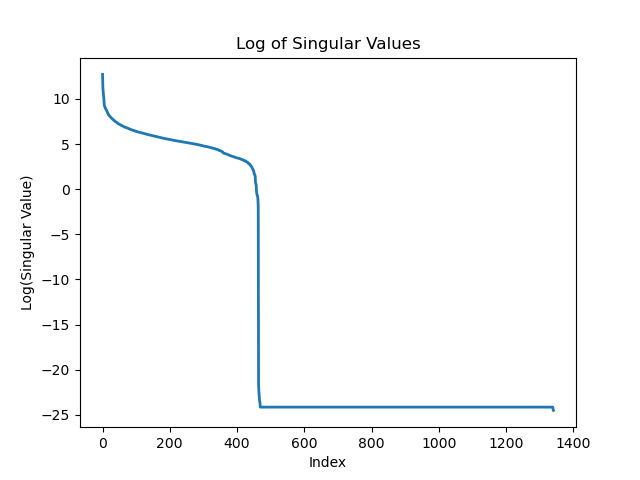
\includegraphics[width=\linewidth]{./code/singular_values_plot.png}
\subcaption{log plot of singular values}
\end{subfigure}
\end{figure}

\begin{figure}[H]
\centering
\begin{subfigure}{0.3\textwidth}

\includegraphics[width=\linewidth]{./code/compressed_rank_10.png}
\subcaption{rank 10}
\end{subfigure}
\begin{subfigure}{0.3\textwidth}
    
\includegraphics[width=\linewidth]{./code/compressed_rank_20.png}
    \subcaption{rank 20}
    \end{subfigure}
    \begin{subfigure}{0.3\textwidth}
        
\includegraphics[width=\linewidth]{./code/compressed_rank_30.png}
        \subcaption{rank 30}
        \end{subfigure}
\end{figure}


\section{QR}
We simplify the demonstration by assuming $A$ is full rank and has eigenvalues $|\lambda_1|>|\lambda_2|>\cdots>|\lambda_n|$.
\subsection{}
For any matrix $A\in \sR^{n\times n}$, with $A=QR$. $a_1,a_2,\cdots,a_n$ are columns of $A$ and $q_1,q_2,\cdots,q_n$ are columns of $Q$. Show that for any k, space spann by $a_1,\cdots,a_k$ is the same as $q_1,\cdots,q_k$.

\subsection{}
try to undersand the following iteration, Argure that $Q_k$ converges to $Q$ 
$$
\begin{aligned}
    &\hat{Q}_0=I, \\ 
    &B_1=A\hat{Q}_0,\\ 
    &\hat{Q}_1\hat{R}_1=B_1,\\ 
    &B_2=A\hat{Q}_1,\\
    &\hat{Q}_2\hat{R}_2=B_2,\\
    &B_2=A\hat{Q}_2,\\
    &\cdots
\end{aligned}
$$


\subsection{}
compare above iteration with QR iteration, Argue that $\hat{Q}_k=Q_kQ_{k-1}\cdots Q_1$ 
$$
\begin{aligned}
    &A_1=A, \\ 
    &A_1=Q_1R_1\\ 
    &A_2=R_1Q_1\\
    &A_2=Q_2R_2\\
    &A_3=R_2Q_2\\
    &\cdots
\end{aligned}
$$



\end{document}